\documentclass[10pt]{article}
\usepackage[margin=2cm]{geometry}
\usepackage{booktabs}
\usepackage{graphicx}
\usepackage{hyperref}
\usepackage{amsmath}

\begin{document}

\title{CSCI 5942: AI Engineering Assignment 3\\Data Pipelines}
\author{Bill Hsu}
\maketitle

% =====================================================================
\section{Data Analysis}

The graded corpus was built from five Common Crawl WET files
(\texttt{data/raw}, 380\,MB gzipped) in 115\,s on a local Spark session.
Table~\ref{tab:funnel} reports the per-stage line counts and sizes. 


\begin{table}[htbp]
\caption{Pipeline funnel over the graded corpus. Percentages are relative
to the line count after chunking.}
\label{tab:funnel}
\centering
\begin{tabular}{lrrr}
\toprule
Stage & Rows & \% of lines & MB \\
\midrule
1 ingest      & 116{,}771    & ---    & 1073.2 \\
2 chunk       & 22{,}461{,}175 & 100.00 & 1050.2 \\
3 normalize   & 19{,}024{,}390 & 84.70  & 684.6 \\
4 features    & 19{,}024{,}390 & 84.70  & 684.6 \\
5 exact dedup & 6{,}093{,}868  & 27.13  & 437.6 \\
6 write       & 6{,}093{,}868  & 27.13  & 437.6 \\
\bottomrule
\end{tabular}
\end{table}

From the table, the most aggressive filter is exact dedup, which removes
68\% of the surviving lines. This indicates that web text contains a 
significant amount of duplicate content, likely due to repeated navigation 
elements, advertisements, and other boilerplate text across different pages. 
The normalize stage, while only dropping 15\% of rows, reduces the byte size 
by 35\%, suggesting that many lines are being shortened or cleaned up, which
is consistent with the fact that \texttt{A1\_VOCAB} has a limited character set
and lacks digits except for '3'.


Table~\ref{tab:features} summarises the feature columns over all
6{,}093{,}868 lines of the finished corpus. I added \texttt{line\_freq} features,
which counts how many times each line's exact text occurs in the corpus.
From the statistics like \texttt{n\_chars} and \texttt{n\_words} we can tell 
that the corpus is mostly composed of short fragments, with a thin tail of 
very long lines that carry most of the characters. The median values are significantly 
lower than the mean values, indicating a skewed distribution. Also, the \texttt{stop\_hits} 
feature has a median of 0, which might not be an ideal feature for filtering as most of the lines
do not contain any of the six English function words. Finally, only 17.67\% of lines end 
in terminal punctuation, indicating that the majority of the corpus does not consist of complete sentences.

I choose to add \texttt{line\_freq} because it provides a direct measure of repetition in the corpus.
Lines that appear frequently are likely to be navigation labels, cookie banners, etc,
which might not be useful for training a language model. We will discuss this feature later in the report.


\begin{table}[htbp]
\caption{Feature statistics of the corpus. \texttt{line\_freq} counts the number of times each line's exact text occurs in the corpus. \texttt{ends\_sentence} is boolean and true for
17.67\% of lines. Computed with a separate analysis script that reads
\texttt{out/raw/corpus}; it is not part of the pipeline.}
\label{tab:features}
\centering
\begin{tabular}{lrrrr}
\toprule
Feature & min & median & mean & max \\
\midrule
\texttt{doc\_stopwords} & 0.00 & 5.00 & 3.80 & 6.00 \\
\texttt{doc\_lines}     & 3.00 & 264.00 & 718.68 & 21{,}508 \\
\texttt{doc\_mean\_line} & 2.65 & 29.90 & 46.30 & 314{,}508 \\
\texttt{line\_ix}       & 0.00 & 104.00 & 340.16 & 21{,}268 \\
\texttt{n\_chars}       & 1.00 & 24.00 & 71.82 & 960{,}960 \\
\texttt{n\_words}       & 1.00 & 4.00 & 9.99 & 141{,}153 \\
\texttt{alpha\_ratio}   & 0.00 & 0.86 & 0.85 & 1.00 \\
\texttt{upper\_ratio}   & 0.00 & 0.11 & 0.15 & 1.00 \\
\texttt{stop\_hits}     & 0.00 & 0.00 & 0.40 & 6.00 \\
\texttt{word\_len\_mean} & 1.00 & 5.57 & 6.86 & 787{,}955 \\
\texttt{rel\_pos}       & 0.00 & 0.46 & 0.47 & 1.00 \\
\texttt{line\_freq}     & 1.00 & 1.00 & 3.12 & 198{,}542 \\
\bottomrule
\end{tabular}
\end{table}

% TODO(you): write a paragraph on Table~\ref{tab:features}. The columns
% worth commenting on, all checkable from the table:
%
%  - The maxima are the story. One "line" is 960,960 characters; one
%    "word" averages 787,955 characters, which only happens when a line
%    contains no spaces at all -- minified JavaScript. One line repeats
%    198,542 times.
%  - The medians are tiny next to the means: n_chars is 24 at the median
%    against a mean of 71.82. The corpus is mostly short fragments with a
%    thin tail of very long lines that carries most of the characters.
%  - stop_hits has a median of 0: most lines contain none of the six
%    English function words at all.
%  - Only 17.7% of lines end in terminal punctuation, so the majority of
%    the corpus is not sentences.
%
%  (a) Which stage filtered the most, and what that says about web text.
%      Exact dedup removes 68% of the surviving lines -- by far the
%      largest single cut.
%  (b) Normalize drops only 15% of ROWS but 35% of BYTES. Explain the
%      gap: most lines survive but lose characters in-line, because
%      A1_VOCAB has 65 characters and no digits except '3'.
%  (c) Feature statistics: report df.describe() on the feature columns
%      and comment on what the extremes reveal.

% TODO(you): insert your own df.describe() output as a table here, and
% comment on at least two columns.

% =====================================================================
\newpage
\section{The Grid}

Every mix is a query over the catalog plus the fixed 50\,M token budget,
so the eight runs differ only in \emph{which} tokens the model saw.
Table~\ref{tab:mixes} gives the mix definitions, the pool each query
leaves and the realised token count after the cut to budget;
Table~\ref{tab:grid} gives the evaluation grid.


\begin{table}[htbp]
\caption{Mix definitions, pool size before the budget cut, and realised
token counts. Every mix trains on the same 50\,M tokens; the pool only
determines how much the sampler had to choose from.}
\label{tab:mixes}
\centering
\small
\begin{tabular}{llrrr}
\toprule
Mix & Query & Pool & Rows & Tokens \\
\midrule
\texttt{baseline}           & \texttt{true} & 437.6\,M & 714{,}946 & 49.9\,M \\
\texttt{english\_pages}     & \texttt{doc\_stopwords >= 5} & 259.2\,M & 589{,}555 & 50.1\,M \\
\texttt{position\_only}     & \texttt{rel\_pos in [0.2, 0.8]} & 255.2\,M & 743{,}349 & 50.0\,M \\
\texttt{stop3}              & \texttt{doc\_stopwords >= 3} & 306.5\,M & 628{,}179 & 49.8\,M \\
\texttt{stop3\_mid}         & \texttt{doc\_stopwords >= 3 AND rel\_pos in [0.2, 0.8]} & 177.9\,M & 666{,}812 & 50.0\,M \\
\texttt{stop3\_mid\_narrow} & \texttt{doc\_stopwords >= 3 AND rel\_pos in [0.3, 0.7]} & 121.4\,M & 666{,}840 & 50.2\,M \\
\texttt{stop4\_mid\_narrow} & \texttt{doc\_stopwords >= 4 AND rel\_pos in [0.3, 0.7]} & 111.7\,M & 651{,}899 & 50.1\,M \\
\texttt{narrow\_line\_freq} & \texttt{line\_freq <= 5 AND doc\_stopwords >= 4 AND rel\_pos in [0.3, 0.7]} & 110.3\,M & 632{,}453 & 50.0\,M \\
\bottomrule
\end{tabular}
\end{table}

\begin{table}[htbp]
\caption{Evaluation grid, nats/char (lower is better). Best per column in bold.}
\label{tab:grid}
\centering
\begin{tabular}{lrrrr}
\toprule
Mix & wikipedia & tinystories & shakespeare & python-code \\
\midrule
\texttt{baseline}           & 1.8665 & 1.9449 & 2.8188 & 3.2683 \\
\texttt{english\_pages}     & 1.7931 & 1.8659 & 2.7361 & 3.2566 \\
\texttt{position\_only}     & 1.6798 & 1.7797 & 2.6563 & 3.1769 \\
\texttt{stop3}              & 1.8536 & 1.9193 & 2.8454 & 3.5303 \\
\texttt{stop3\_mid}         & 1.6251 & 1.7405 & 2.7134 & 3.0997 \\
\texttt{stop3\_mid\_narrow} & 1.5860 & 1.7034 & 2.6691 & \textbf{2.9851} \\
\texttt{stop4\_mid\_narrow} & \textbf{1.5757} & 1.6812 & \textbf{2.6489} & 3.2830 \\
\texttt{narrow\_line\_freq} & 1.5759 & \textbf{1.6762} & 2.6700 & 3.2975 \\
\bottomrule
\end{tabular}
\end{table}

Three pairs in Table~\ref{tab:grid} differ in exactly one predicate, so
each isolates the contribution of a single filter on wikipedia:

\begin{table}[htbp]
\caption{Controlled contrasts on wikipedia. Negative is an improvement.}
\label{tab:contrasts}
\centering
\begin{tabular}{llr}
\toprule
Change & Pair & $\Delta$ \\
\midrule
\texttt{rel\_pos} [0.2,0.8] $\to$ [0.3,0.7] & \texttt{stop3\_mid} $\to$ \texttt{stop3\_mid\_narrow} & $-0.0391$ \\
\texttt{doc\_stopwords} 3 $\to$ 4            & \texttt{stop3\_mid\_narrow} $\to$ \texttt{stop4\_mid\_narrow} & $-0.0103$ \\
add \texttt{line\_freq <= 5}                 & \texttt{stop4\_mid\_narrow} $\to$ \texttt{narrow\_line\_freq} & $+0.0002$ \\
\bottomrule
\end{tabular}
\end{table}

\begin{figure}[htbp]
\centering
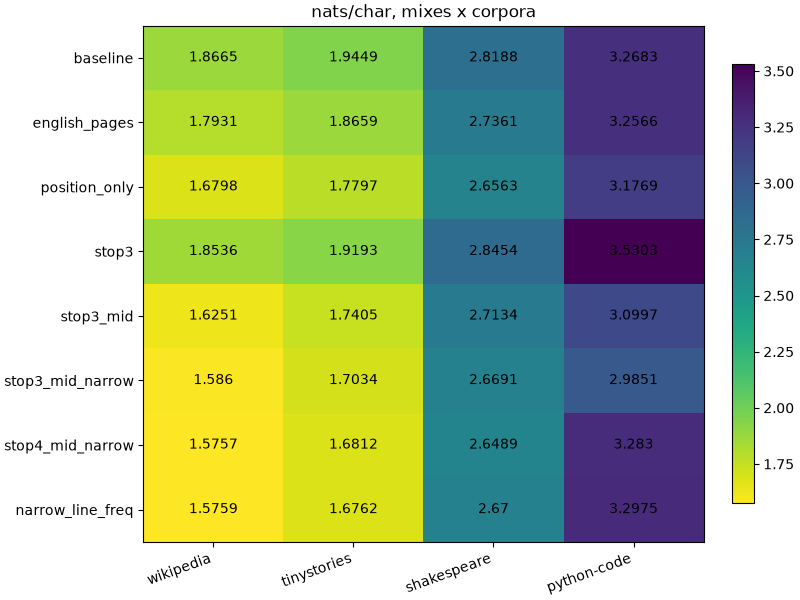
\includegraphics[width=\textwidth]{eval/results/heatmap.png}
\caption{Evaluation grid as a heatmap. Lighter is better.}
\label{fig:heatmap}
\end{figure}

\newpage
% =====================================================================
\section{Analysis of the Best Mix}


\texttt{stop4\_mid\_narrow} reaches 1.5757 nats/char on wikipedia, an
improvement of 0.291 over \texttt{baseline} (1.8665) and 0.217 over the
\texttt{english\_pages} reference (1.7931), at an identical token budget.

Both of the queries are page-level. \texttt{doc\_stopwords >= 4} keeps
lines from pages that contain at least four of the six English function
words anywhere in the page; \texttt{rel\_pos} in $[0.3, 0.7]$ keeps only
the middle 40\% of each page.

Table~\ref{tab:contrasts} shows the position band is doing most of the
work: tightening \texttt{rel\_pos} is worth $-0.0391$ while raising the
language threshold from three to four is worth $-0.0103$, four times
less.

My assumption is that the position filter is removing boilerplate, which is
often clustered at the top and bottom of pages, while the stopword filter
is removing pages that are not English prose. The two filters are complementary:
the position filter removes low-quality lines from otherwise good pages,
while the stopword filter removes entire pages that are not English prose.

\subsection*{The other corpora}

The three prose corpora move together: every mix that improves wikipedia
improves tinystories and shakespeare by a similar margin, which is what
one would expect if the filters are selecting for well-formed English
rather than for anything wikipedia-specific.

However python-code does not follow. Its best score in the grid belongs to
\texttt{stop3\_mid\_narrow} (2.9851), not to the wikipedia winner:
raising \texttt{doc\_stopwords} from three to four buys $0.0103$ on
wikipedia and costs $0.298$ on python-code.

From the results, the trade-off is clear: a stricter page-level English filter
removes code-related data, which carry few English function words, so the training
distribution moves toward English prose and away from code. The model
sees less code and performs worse on python-code. The trade-off is between
improving performance on English prose and degrading performance on code.


% TODO(you): explain that trade-off. The mechanism worth arguing: a
% stricter page-level English filter removes code-heavy pages, which
% carry few English function words, so the model sees less code.
% Generalise it -- moving the training distribution toward one target
% moves it away from others.

% =====================================================================
\section{What Did Not Work}

Two of my mixes did not work. The first one is \texttt{stop3}. The
second one uses my custom feature \texttt{line\_freq}.

\subsection*{\texttt{stop3}: a weaker filter}

\texttt{stop3} keeps every page with three or more of the six stopwords.
It scored 1.8536 on wikipedia. That is worse than
\texttt{english\_pages} (1.7931). It is also very close to no filter at
all (1.8665).

The reason is simple. \texttt{english\_pages} uses
\texttt{doc\_stopwords >= 5}. My filter uses \texttt{>= 3}, so it is
easier to pass. More pages get in. The pool shows this: 306.5\,M tokens
for \texttt{stop3}, but only 259.2\,M for \texttt{english\_pages}. My
filter keeps 70\% of the corpus, so it removes almost nothing.

\texttt{english\_pages} already showed that removing non-English pages
helps. I made the same filter weaker, so the result moved back toward
the baseline.

On python-code, \texttt{stop3} was the worst mix in the grid: 3.5303,
worse than no filter (3.2683). A page of code has very few English
stopwords. So \texttt{doc\_stopwords >= 3} removes code pages, but keeps
most other bad lines. The model saw less code and did not get anything
useful back.

This mix was not a good idea, however it was useful for comparison with
other mixes like \texttt{stop3\_mid} and \texttt{stop3\_mid\_narrow}, 
which use the same \texttt{doc\_stopwords >= 3} filter but add a position filter.


\subsection*{\texttt{narrow\_line\_freq}: no effect}

The second mix adds \texttt{line\_freq <= 5} to my best mix. It scored
1.5759 on wikipedia. My best mix scored 1.5757. The difference is
0.0002, which is nothing. Section~\ref{sec:part1} explains why.
\newpage
% =====================================================================
\section{Changes to Part 1}
\label{sec:part1}

\subsection*{The feature}

A extra stage, \texttt{stage\_user\_line\_freq}, adds \texttt{line\_freq}:
how many times a line's exact text occurs anywhere in the corpus. It sits
between the feature stage and exact dedup, because dedup collapses the
duplicates.

\subsection*{Why the existing signals were not enough}

Exact dedup already removes duplicates. It cut 19.0\,M lines down to
6.1\,M, which is 68\% of the corpus. But dedup only keeps one copy. It
does not save how many copies there were. After this stage, a line that
appeared three thousand times looks the same as a line that appeared
twice.

My assumption is that a line with many copies is usually boilerplate,
like a menu item or a cookie message. A line with one copy is more
likely to be real content. If I know the count, I can use it to remove
this type of text.


\subsection*{What happened}

\texttt{narrow\_line\_freq} adds \texttt{line\_freq <= 5} to my best
mix. On wikipedia it changed the score by $+0.0002$. That is no effect.

Table~\ref{tab:features} already shows a warning sign. The median of
\texttt{line\_freq} is 1, but the mean is 3.12 and the max is 198{,}542.
So a small number of lines repeat a huge number of times, and most lines
do not repeat at all.

Table~\ref{tab:freq} explains the result. Repeated lines are short. Lines
that repeat 11 times or more are 2.3\% of all lines, but only 0.7\% of
all characters. Their average length is 22 characters. The top of the
list is even shorter: \texttt{'3'} appears 198{,}542 times,
\texttt{'.'} appears 129{,}600 times, and \texttt{'Home'} appears
50{,}883 times.

\begin{table}[htbp]
\caption{Lines grouped by \texttt{line\_freq}, over the full corpus.
Repeated lines are many, but they are short, so they hold few
characters. Computed with a separate analysis script that reads
\texttt{out/raw/corpus}; it is not part of the pipeline.}
\label{tab:freq}
\centering
\begin{tabular}{lrrrr}
\toprule
\texttt{line\_freq} & lines & \% of lines & \% of chars & mean chars \\
\midrule
1     & 3{,}950{,}381 & 64.8\% & 82.1\% & 91 \\
2--5  & 1{,}781{,}772 & 29.2\% & 15.9\% & 39 \\
6--10 & 218{,}584     & 3.6\%  & 1.3\%  & 26 \\
11+   & 143{,}131     & 2.3\%  & 0.7\%  & 22 \\
\bottomrule
\end{tabular}
\end{table}

The budget is 50\,M \emph{characters}, not 50\,M lines. This is the
problem. My filter \texttt{line\_freq <= 5} keeps 98.0\% of all
characters, so it only removes 2.0\% of the budget. It cannot change the
mix very much.

There is a second problem. Repeated does not always mean bad. Normal
English can repeat on many websites, for example when an article is
copied or quoted. A stricter threshold would remove this good text
together with the boilerplate, like menus and headlines.

To conclude, the feature is straightforward and cheap to compute, and it
does find repeated text. The problem is that the repeated text it finds
is too short to matter at this budget.

\end{document}
